
\section{Obrazowe techniki diagnostyczne}
Istnieje wiele technik obrazowania wykorzystujące różne zjawiska fizyczne zachodzące w materii.
Podstawowe techniki obrazowania medycznego to:
\label{sec:basic-imaging-technics}
\begin{itemize}
    \item Radiografia - RTG

    Radiografia to najstarsza i najbardziej rozpoznawalna technika obrazowania.
    Pierwsze zdjęcie analogowe zostało wykonane przez Röntgena w 1896 roku.
    Polega na transmisji promieniowania X przez badany obiekt, a następnie detekcji tego promieniowania za obiektem badanym.
    Promieniowanie za obiektem jest funkcją współczynnika osłabiania promieniowania rentgenowskiego dla materii znajdującej się na drodze tego promieniowania.
    Wyróżniamy dwa typy radiografii: analogową i cyfrową.
    Radiografia analogowa wykorzystująca naświetlanie filmów światłoczułych odchodzi powoli w zapomnienie ze względu na koszt i uciążliwość wywoływania filmów.
    \todo {WS: powtórzenie z analogówki; jakie dwa typy detektorów są stosowane? }
		W radiografii cyfrowej obrazowana jest ilość promieniowania X przenikające przez badany obiekt.
    
		\todo {WS podać ogólne cechy obrazu!!!; }
		Kontrast zależy od położenia obiektu między źródłem a detektorem (położenie optymalne), napięcie anodowe, filtracja, grubość okładek wzmacniających.
    \todo {WS: masło jest maślane; }
		Rozdzielczość zależy od rozdzielczości detektora i rozmiaru ogniska lampy.
    
    W standardzie DICOM radiografia cyfrowa jest oznaczana jako \quotett{RT}.

    \item Tomografia komputerowa (Computer Tomography - CT)
    
    \todo {agregacja?! }Akwizycja w tomografii komputerowej jest podobna do badania RTG, ale w CT wykonujemy wiele pomiarów w różnych pozycjach względem obiektu badanego i pod różnym kątem.
		W tomografii komputerowej podobnie jak w radiografii wykorzystuje się promieniowanie X do pomiaru projekcji (stąd inna nazwa tomografia rentgenowska). W wybranej płaszczyźnie dokonuje się pomiarów projekcji po liniach biegnących pod różnym kątem i w różnych odległościach od badanego obiektu. Przekrój obiektu jest rekonstruowany numerycznie na podstawie zmierzonych projekcji projekcji.
    \todo {tworzymy tworzący? }
		Następnie z tych pomiarów tworzymy obraz przez zastosowanie odpowiednich algorytmów tworzących obraz.
    Rejestrujemy współczynnik osłabienia promieniowania rentgenowskiego przez badany obiekt.
\todo {WS: to już było i jest bez większego znaczenia dla pracy; jakie są obrazy? rozdzielczość przestrzenna, próbkowanie, kwantyzacja? }
    Kontrast zależy od rozmiarów szczegółów badanego obiektu, napięcie anodowe, przyłożone masy (prąd katodowy i czas akwizycji).\todo {jakie mAs-y? prąd na lampie? }
    Rozdzielczość zależy od geometrii pomiaru, rozmiaru ogniska lampy rentgenowskiej, przestrzenna rozdzielczość matrycy detektora, liczby detektorów, dyskretyzację i filtru rekonstrukcyjnego.

    W standardzie DICOM technika jest oznaczana skrótowcem \quotett{CT}.

    \item Obrazowanie metodą rezonansu magnetycznego - MRI

    Sposób tworzenie obrazu MRI jest wysoce skomplikowanym procesem i ciężko opisać go w kilku zdaniach.
		\todo {to zależy od sekwencji! są obrazy PD, T1 i T2; }Obrazowana jest sumaryczna gęstość atomów wodoru (protonów) w badanym obiekcie.
    Kontrast zależy od gęstości protonów, czasu relaksacji podłużnej i poprzecznej, prędkości przepływu płynu.
    \todo {są obrazy statyczne ale też dynamiczne ; są też obrazy pokazujące funkcje (fMRI); te są pokazywane w innej skali barwnej}
		Rozdzielczość zależy od parametrów skanera (rozmiar woksela).
    
    W standardzie DICOM modalność rezonansu magnetycznego jest oznaczana jako \quotett{MR}.
    
    \item Ultrasonografia
    
    Jest to badanie, które wszyscy kojarzą z badaniem płodu podczas ciąży z obrazem w kształcie łuku na, którym nic nie widać.\todo {usunąć to zdanie} 
    Badanie ultrasonograficzne polega na wygenerowaniu fali akustycznej o wysokich częstotliwości, a następnie wprowadzeniu jej do ciała pacjenta.\todo {niefortunne 'wprowadzenie'; tu powinno by c coś o odbiciu} 
    Następnie nasłuchuje się echa po tej fali.
    Obrazowana jest odbita fala ultradźwiękowa, osłabienia po odbiciach, zmienna częstotliwość i opóźnienie w czasie.\todo {od czago zależy położenie, a od czego wielkość sygnału}
    Kontrast zależy od częstotliwości fali, głębokości badanego obiektu, ilości piezoelektryków w głowicy, obrazowanej struktury.
    Rozdzielczość zależy od czasu trwania impulsu zaburzenia oraz od szerokości wiązki ultradźwiękowej (powierzchnia czynna przetworników).

    W standardzie DICOM obraz ultrasonograficzny jest oznaczana jako \quotett{US}.\todo {mamy też obrazy doplerowskie; jak są zapisywane w DICOM?}

    \item Scyntygrafia
    
    Obrazowa technika diagnostyczna z gałęzi medycyny nuklearnej.
    Polega na wprowadzenia do organizmu \todo {to nie są ciała obce, środków chemicznych} radiofarmaceutyków znakowanych izotopem, \todo {izotop, którym znakowany jest farmacuetyk ma tę cechę}charakteryzującym się krótkim czasem rozpadu i powinowactwem chemicznym z badanymi organami.
    Następnie wykrywanie rozpadów zachodzących w ciele poprzez rejestracje promieniowania wytwarzanego podczas rozpadu, a następnie przedstawienie to w formie graficznej. \todo {detekcja}
    Kontrast zależy od czasu trwania pomiaru, oraz od aktywności wstrzykniętego radiofarmaceutyka.
    Rozdzielczość zależy od ułożenia \todo {ułożenia???} i możliwości rozdzielczej \todo {znowu masło maślane} kamer scyntylacyjnych, zwanymi także scyntykamerami, gammakamerami lub kamerami Angera.

    W standardzie DICOM obraz scyntygraficzny jest oznaczana jako \quotett{NM}.

    Radiofarmaceutyki to związki chemiczne zawierające radioizotop.

    \item Tomografia SPECT
    
    Technika obrazowania  z gałęzi medycyny nuklearnej, w której rejestruje się promieniowanie powstające rozpadu gamma.
    Źródłem promieniowania(fotonów) jest podany pacjentowi radiofarmaceutyk, ulegająca rozpadowi gamma.
    Rejestrujemy fotony powstające podczas anihilacji pozytonów.
    Kontrast zależy od wydajności detektorów, odległość detektora od obiektu oraz położenie obiektu.
    Na rozdzielczość ma wpływ przestrzenna rozdzielczość matrycy detektora, liczby detektorów.

    W standardzie DICOM obraz ultrasonograficzny jest oznaczana jako \quotett{PT}.

    \item Tomografii PET
    
    Technika obrazowania  z gałęzi medycyny nuklearnej. w której rejestruje się promieniowanie powstające podczas anihilacji pozytonów (antyelektronów).
    Źródłem promieniowania(pozytonów) jest podana pacjentowi substancja promieniotwórcza, ulegająca rozpadowi beta plus.
    Rejestrujemy fotony powstające podczas anihilacji pozytonów.
    Kontrast zależy od wydajności detektorów, odległość detektora od obiektu oraz położenie obiektu.
    Na rozdzielczość ma wpływ przestrzenna rozdzielczość matrycy detektora, liczby detektorów.

    W standardzie DICOM obraz ultrasonograficzny jest oznaczana jako \quotett{PT}.
    
\end{itemize}

Istnieją też techniki, które są połączeniem kilku innych technik.
Takie jak:
\begin{itemize}
    \item PET-CT, PET/CT - połączenie PET z wielorzędowym tomografem komputerowym
    \item PET-MRI, PET/MRI - połączenie PET z rezonansem magnetycznym
\end{itemize}

Standard DICOM nazywa techniki obrazowania modalnościami(z ang. modality).

\section{Obrazy diagnostyczne}

\subsection{Parametry obrazów}

\subsubsection{Wartość diagnostyczna obrazu}

W obrazowaniu medycznym chodzi o wyciągnięcie wniosków z obrazów i postawienie diagnozy.
Jest to kluczowy element obrazowania.
Brak możliwości stwierdzenia co na obrazie się znajduje, stawia sens takiego obrazowania pod znakiem zapytania.
Poco nam obraz w 4K na, którym można zobaczyć wyraźne plamy niczego.

Wartość diagnostyczną można określić na podstawie następujących parametrów
\begin{itemize}
    \item Jakości obrazu
    
    Parametry jakościowe obrazów są szczegółowo opisane w sekcji \ref{sec:image-quality}

    \item Warunków obserwacji obrazu

    W brew pozorom warunki obserwacji mają kluczowe znaczenie dla wartości diagnostycznej.
    Jeżeli będziemy mieli dobry obraz, który wyświetlimy na budżetowym monitorze RGB, który w rzeczywistości posiada 6-bite kanały RGB i tworzy odcienie za pomocą techniki dithering'u, to niewiele zobaczymy.

    \item wiarygodności diagnostycznej obrazów

    \item charakterystyki pracy lekarza-specjalisty

\end{itemize}

\subsubsection{Jakość obrazów}
\label{sec:image-quality}

\begin{itemize}
    \item Kontrast
    
    ???

    kontrast mikelsona

    max-min / max+min
    
    amplidua sinusoidy do wartości średniej

    \item Rozdzielczość przestrzenna

    Rozdzielczość przestrzenna obrazu to najmniejsza odległość między dwoma punktami obrazu, które można rozróżnić.
    W radiografii rozdzielczość określa się zazwyczaj jako liczbę równoległych linii, czarnych i białych, które można rozróżnić ma 1 milimetrze obrazu(paralinie na milimetr).

    Porównanie zdolności rozdzielczych różnych technik obrazowania:
    \begin{itemize}
        \item scyntygrafia - 
        \item USG - 
        \item MRI -
        \item CT -
        \item radiografia -
    \end{itemize}
    TUTAJ COŚ WPISAĆ

    rozdzielczośc przy przy kontraście

    \item Stosunek sygnału użytecznego do szumu (SNR)

    W obrazach zawsze występuje szum, widoczny w różnych postaciach, na przykład w postaci cyfrowego ziarna.
    Rodzaj i poziom szumu zależy od techniki obrazowania.
    Stosunek sygnału użytecznego ma decydujący wpływ na widoczności obiektów, kontrast oraz percepcję szczegółów w obrazie.

    \item Poziom artefaktów
    
    Artefakty to zjawiska fałszujące obraz poprzez tworzeni nie istniejących struktur w obrazie.
    Problemem występującym w różnych technikach obrazowania.
    Najbardziej widocznymi artefaktami są warkocz komety i odbicie zwierciadlane w obrazach USG.

    \item Poziom zniekształceń przestrzennych
    
    Zniekształcenia przestrzenne powstają w wyniku geometrycznego ułożenia i kształtu obiektu badanego i aparat pomiarowego.
    Przykładem takiego zniekształcenia mogą być różne powiększenia obiektów zależne od głębokości ich ułożenia w USG, zmiana pozycji pacjenta(przez ruchy klatki piersiowej w czasie badani), czy deformacja obrazu spowodowana zmianami rozkładu pola magnetycznego przez metalowe obiekty w znaldujące się w tym samym pomieszczeniu, co MRI.

\end{itemize}

\section{Zapisywanie obrazów i standard DICOM}
\subsection{Standard DICOM v3.0}

\par
Standard DICOM jest odpowiedzią społeczności radiologów, radiofarmaceutów, fizyków medycznych na potrzebę wymiany danych pomiędzy różnymi systemami komputerowymi, przeglądarek obrazów,  stacji do przetwarzania i analizowania obrazów medycznych.

\par
Standard DICOM wersji trzeciej to standard definiujący ujednolicony sposób zapisu i przekazywania danych medycznych reprezentujących lub związanych z obrazami diagnostycznymi w medycynie.
Standard został wydany w 1993 przez dwie agencje ACR (American College of Radiology) i NEMA (National Electrical Manufactures Association).
Wcześniejsze wersje nazywały się ACR/NEMA v1.0, wydana w 1983 roku i ACR/NEMA v2.0, wydana w 1990 roku, stąd wersja trzecia.
Od wydania wersji trzeciej w 1993, standard jest wciąż rozwijany i uzupełniany o nowe elementy.
W obecnej chwili standard DICOM definiuje 81 różnych typów badań.

UWAGA: Za każdym razem kiedy jest odniesienie do obecnego standardu DICOM, w domyśle jest to odsłona 2019a.

\subsection{Sposób zapisu danych w pliku DICOM}

\par
Plik w formacie DICOM przypomina zbiór \enquote{elementów danych} z rekordami.
Zbiór nazywa się \keyword{Data Set} i składa się z rekordów, które nazywają się \keyword{Data Element}.
Elementy danych są ułożone w postaci listy.
Element danych może zawierać w sobie listę elementów danych.

\begin{figure}[!htbp]
    \centering
    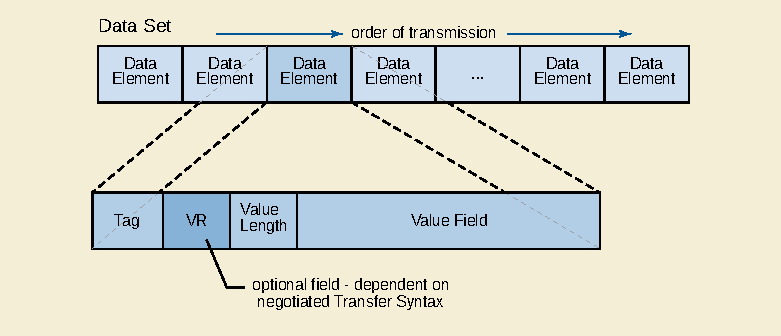
\includegraphics[]{img/dicom-dataelement001.pdf}
    \caption{Elementy danych w zbiorze elementów danych}
    \label{fig:dicom-dataelement}
\end{figure}

\subsubsection{Data Element}

\keyword{Data Element} jest rekordem, który przechowuje jakaś jedną informacje o czymś.
Składa się z czterem elementów:

\begin{itemize}

    \item \keyword{Tag} - to unikalny identyfikator, dalej zwany zanczniekiem, złożony z dwóch liczb: numer grupy (\cppcode{uint16}) i numer elementu (\cppcode{uint16}) grupy.
          Informuje o tym co dany rekord w sobie zawiera.
          W jednym zbiorze elementów nie mogą się pojawić dwa elementy posiadających ten sam znacznik.

          Na przykład: jeżeli liczby \keyword{Tag} przyjmą wartości odpowiednio wartość $0010_{16}$ i $0010_{16}$ to oznacza, że jest to tag \dicomtag{PatientName}{0010}{0010}, czyli zwiera w sobie parametr zawierają nazwę pacjenta.

          Dokładne omówienie \keyword{Tag}-ów znajduje się w dalszej części sekcji.

    \item \keyword{Value Representation}, w skrócie \keyword{VR} – to dwa bajty w postaci tekstu, informujący o formacie w jaki parametr został zapisany.

          Dokładne omówienie \keyword{VR}-ów znajduje się w dalszej części sekcji.

    \item \keyword{Value Length}, w skrócie \keyword{VL} - 32-bitowa lub 16-bitowa liczba nieoznaczona, która informuje o długości pola danych (\keyword{Value Field}).

          Wartość \keyword{VL} zwykle jest liczbą parzystą.
          Standard DICOM zakłada, że wszystkie dane powinny być dopełniane do parzystej liczby bajtów.

    \item \keyword{Value Field} (opcjonalne) - pole z parametrem o długości VL.

\end{itemize}

\subsubsection{Znacznik}
\label{sec:dicom-tag}

Tagi to unikalne znaczniki pozwalające określać co jest zapisane w \keyword{Data Element}.
Tag jest zrobiony z dwóch liczb: numeru grupy i numeru elementu.
Obie liczby to 16-bitowe liczby całkowite zapisywane w postaci  heksadecymalnej.

Istnieją dwa rodzaje znaczników: publiczne o parzystym numerze grupy i prywatne o nieparzystym numerze.
Pierwsza grupa jest definiowana przez standard DICOM, zawiera ona podstawowe znaczniki
Publiczne znaczniki dzielę się na obowiązkowe, opcjonalne i warunkowe.
Są określane przy definicji obiektów informacyjnych.
Natomiast druga grupa to tagi, pozostawione do dyspozycji producentom sprzętu, tak by mogli zapisywać dodatkowe informacje, które nie zostały przewidziane w standardzie DICOM.
Taki umożliwia podział umożliwia zapisywane ogromnej liczby informacji ustandaryzowanej jak i informacji niestandardowej w sposób bezkonfliktowy i z możliwosćią odczytania danych przez aplikacje nie związane z producentem sprzętu.

Obecna odsłona DICOM definiuje znaczenie ponad 4000 publicznych tagów z informacjami oraz jakie VR powinny mieć.
Oto kilka przykładów:
\begin{itemize}
    \item \dicomtag{PatientName}{0010}{0010} - nazwa pacjenta, tag który zawsze musi się pojawić, może być pusty w przypadku kiedy pacjent jest bezimienny

    \item \dicomtag{PatientID}{0010}{0020} - id pacjenta, unikalny identyfikator pacjenta, najczęściej jest to numer HIS(Hospital Information System)

    \item \dicomtag{PatientBirthDate}{0010}{0030} - data urodzenia pacjenta

    \item \dicomtag{PatientSex}{0010}{0040} - płeć pacjenta

    \item \dicomtag{PatientAge}{0010}{1010} - wiek pacjenta w czasie badania

    \item \dicomtag{StudyDescription}{0008}{1030} - opis badania, pole wypełniane przez technika lub lekarza

    \item \dicomtag{SeriesDescription}{0008}{103E} - ops serii, pole wypełniane przez technika lub lekarza

    \item \dicomtag{SeriesInstanceUID}{0020}{000E} - unikalny numer serii, jest nadawany każdemu badaniu

    \item \dicomtag{InstanceNumber}{0020}{0013} - numer instancji ramki, używany w przypadku kiedy z jednego badania zostało utworzonych kilka plików DICOM

    \item \dicomtag{Modality}{0008}{0060} - modalność określająca rodzaj techniki diagnostycznej

    \item \dicomtag{StudyDate}{0008}{0020} - data wykonania badania
\end{itemize}


\subsubsection{VR - Value Representation}
\label{sec:dicom-vr}

VR informuje w jakim formacie jest zapisany parametr obrazu.
Składa się z dwóch bajtów.

Przykładowe VR:
\begin{itemize}
    \item AS - Age String - wiek lub długość życia

          Długość danych zawsze wynosi 4 bajty.
          Pierwsze trzy bajty to liczba całkowita zapisana za pomocą tekstu.
          Czwarty bajt to znaku określający jednostkę czasu.
          Standard definiuje cztery możliwe jednostki czasu: \dataword{D} jako dzień, \dataword{W} jako tydzień, \dataword{M} jako miesiąc, oraz \dataword{Y} jako jeden rok.

          Przykład: \dataword{018M} oznacza 18 miesięcy, \dataword{123D} oznacza 123 dni.

    \item AT - Attribute Tag - inny tag

          Długość danych to zawsze 32 bity, są to dwie 16 bitowe liczby.
          Odpowiednio grupa i element grupy.
          Ten VR jest używany kiedy wskazujemy na inny tag.
          Wartość nie jest nigdy pokazywana użytkownikowi, a jedynie używana w interpretacji przez inne algorytmu do analizy obrazu.

          Przykład: tag \dicomtag{FrameIncrementPointer}{0028}{0009} jest używany kiedy w pliku jest zapisana sekwencja kilku obrazów, wskazuje on na inny tag zawierający informacje, w jaki sposób ta sekwencja ma być wyświetlona.

    \item DA - Date - data lub dzień

          Długość danych zawsze wynosi 8 bajtów.
          Data zapisana w formacie \dataword{YYYYMMDD}, gdzie: \dataword{YYYY} cztery cyfry roku, \dataword{MM} dwie cyfry miesiąca, \dataword{DD} dwie cyfry dnia w kalendarzu Gregoriańskim.

          Przykład: \dataword{19800716} oznacza 16 lipca 1980

          UWAGA: Standard \enquote{ACR-NEMA Standard 300}, czyli poprzednik DICOM definiował date w sposób \dataword{YYYY.MM.DD}, według standardu DICOM, taki zapis jest nie poprawny, ale zdarzają się stare obrazy z takimi datami i \sokarclass{DataConverter} obsługuje taki format.

    \item DS - Decimal String - liczba zmiennoprzecinkowa lub ciąg kilku liczb zmienno przecinkowych zapisanych za pomocą tekstu w notacji wykładniczej

          Długość jednej liczby powinna maksymalne wynosić 16 bajtów.
          Dostępne znaki to \dataword{0}-\dataword{9}, \dataword{+}, \dataword{-}, \dataword{E}, \dataword{e}, \dataword{.}.
          Biblioteka QT posiada wbudowany konwerter liczb zapisanych w formacie wykładniczym, dlatego mój konwerter dzieli tekst i konwertuje za pomocą QT.

          Przykład: \dataword{426\textbackslash468 } oznacza dwie liczby 426 i 468. Proszę zwrócić uwagę na spacje na końcu.

    \item IS - Integer String - liczba całkowita

          Długość jednej liczby powinna maksymalne wynosić 12 bajtów.
          Dostępne znaki to \dataword{0}-\dataword{9}, \dataword{+}, \dataword{-}.
          Biblioteka QT posiada wbudowany konwerter liczb całkowitych, dlatego mój konwerter używa konwertera z QT.

          Przykład: \dataword{426 }  oznacza liczbę 426.

    \item PN - Person Name - nazwa osoby

          Jako, że pacjenta, bądź obiekt badany można nazwać w sposób dowolny i odbiegający od polskiego standardu nazewnictwa, standard DICOM nie przewiduje rozdzielenia poszczególnych składowych nazwy na oznaczone fragmenty.
          \enquote{Person Name} dzieli nazwę na podane fragmenty, rozdzielony znakiem \dataword{\^{}} (94 znak kodu ASCII):
          \begin{itemize}
              \item family name complex - nazwisko, np. Smolik
              \item given name complex - imię, np. Adam
              \item middle name - środkowe imię, brak odpowiednika w polskim nazewnictwie
              \item name prefix - prefiks przed imieniem, np: mgr. inż.
              \item name suffix - sufiks po imieniu, brak odpowiednika
          \end{itemize}
          Długość jednego fragmenty powinna maksymalne wynosić 64 znaki.
          W przypadku mniejszej ilości segmentów, mamy założyć, że są puste.

          Przykład: \enquote{prof. dr. hab. inż. Waldemar Smolik pracownik ZEJIM} był by zapisany w sposób następujący: \dataword{Smolik\^{}Waldemar\^{}\^{}prof. dr. hab. inż.\^{}pracownik ZEJIM}

    \item SS - Signed Short - 16 bitowa liczba całkowita bez znaku

    \item US - Unsigned Short - 16 bitowa liczba całkowita ze znakiem

    \item UT - Unlimited Text - tekst o nieograniczonej długości.

          Zwykły tekst o długości maksymalnie $2^{32}-2$ bajtów.
\end{itemize}

\subsection{DICOMDIR}

W przypadku większych instytucji pojawia się problem indeksowania plików i ich przeszukiwania.
Wyszukanie konkretnego badania lub pliku w folderze, w którym znajduje się kilkaset plików poprzez wczytanie pliku i jego odczyt nie jest rozwiązaniem optymalnym.
Dlatego standard DICOM definiuje również pliki typu DICOMDIR, który jest plikiem indeksującym pliki DICOM w folderze.
Pozwala to na efektywne przeglądanie wielu serii badań bez wczytywania plików badań.


\section{Wyświetlanie obrazów}

\par
W celu przeglądania i porównywania należy posiadać jakieś narzędzie do wyświetlenia w sposób poprawny, najlepiej jednym i tym samym programem.
\par
Standard DICOM przewiduje sposób prezentacji danych administracyjnych i danych związanych z rejestracją badania, ajk wyświetlać obrazy radiologiczne i obrazy TK, obrazy scyntylacyjne, itd.

\subsection{Przeglądarki obrazów}

Przeglądarki obrazów to programy należące do kategorii przeglądarki plików.
Zwykłe przeglądarki obrazów takich jak jpg, png lub gif wyświetlają obraz w takiej postaci jakiej jest zapisany, oczywiście najpierw przeprowadzają dekompresje obrazu.
W przypadku obrazów medycznych najczęściej nie mamy do czynienia z danymi reprezentującymi kolory w spektrum światła widzialnego.
Przeglądarka obrazów DICOM musi wygenerować kolorowy obraz z danych na podstawie parametrów obrazu.

\subsection{Funkcje przeglądarek obrazów}

Wyróżniono 26 kryteriów do porównywania przeglądarek w postaci „tak” lub „nie”, podzielonych na 5 grup, platformy, interfejsu, wsparcie, obrazowanie dwu i trój wymiarowego.
Kryteria te w jasny sposób pozwalają na ocenę praktycznych aspektów użytkowania przeglądarki.

\subsubsection{Platforma}

Samodzielność, aplikacje samodzielne są zaprojektowane tak, aby nie wymagały żadnego dodatkowego sprzętu fizycznego bądź infrastruktury do poprawnego działania(np. systemu Windows oraz serwisów przez niego dostarczanych).
Rozwiązania sieciowe, określają czy aplikacja jest usługą sieciową i można z przeglądarki korzystać jak ze strony WWW.
Wieloplatformowość, możliwość uruchomienia ich na różnych systemach operacyjnych Linux/MacOS/Windows
Rozwiązania mobilne, możliwość używania na urządzeniach mobilnych takich jak telefon.

\subsubsection{Interfejs}

Przeglądarka powinna mieć możliwość komunikacji z interfejsami innych systemów.
Podstawowe interfejsy sieciowe to: C-STORE SCP DICOM C-STORE, C-STORE SCU, Query-Retrieve, WADO, Parameter Transfer.

\subsubsection{Wsparcie techniczne}

Dokumentacja, dostępność pisemnej dokumentacji oprogramowania (np. podręczniki lub strony internetowej).
Wsparcie przez pocztę internetową, możliwość porozumienia się z twórcą lub opiekunem oprogramowania.
Forum, możliwość pytania się społeczności o opinie i ich wymiana.
Wiki, strona internetowa w formacie Wikipedii dostępna dla użytkownika.

\subsubsection{Obrazowanie dwu-wymiarowe}

Przewijanie(\fromEng{scroll}), proces wyświetlania obrazów, można poprawić dzięki zmniejszeniu interakcji z klawiaturą oraz myszką. Można to osiągnąć na przykład, oferując możliwość przejścia do następnego lub poprzedniego obrazu przez przesunięcie kółkiem myszy lub używając przycisków góra/dół na klawiaturze.
Metadane, przeglądania powinna obejmować analizowanie i wyświetlanie metadanych obiektów DICOM, powinna obejmować wyświetlanie rozdzielczości obrazu, badanie (np. identyfikator podmiotu) oraz znaczniki DICOM specyficzne dla dostawcy (np. specjalne ustawienie urządzenia rejestrującego).
Warstwa informacyjna, najważniejsze informacje powinny powinny być wizualizowane w oknie wyświetlacza jako nakładka na obraz.
Na przykład aktualna pozycja lub nazwa podmiotu wykonującego badanie.
Okienkowanie (okna cyfrowe), sposób zamiany danych na skale szarości, okienkowanie jest opisane w sekcji \ref{sec:windowing}.
Pseudo-kolorowanie obrazu, tabele (LUT, \fromEng{LookUpTable}) odwzorowujące szare wartości obrazu na pseudo-kolory, poprawiaja one czytelność obrazu.
Histogram, histogramy wizualizują wystąpienia i rozkład wartości kolorów na obrazach, pozwalają opisywać istotne cechy obrazu
Wymiarowanie, możliwości rysowania bądź zaznaczania linii lub innych kształtów do analizy i wyznaczania odległości w jednostkach długości na obrazie.
Jest to możliwe gdyż nagłówki pliku DICOM zawierają parametry sprzętowe urządzenia (np. ilość pikseli na centymetr).
Adnotacje(opisy), które były wytworzone przez personel medyczny powinny być zapisywane w odpowiedni sposób w pliku.

\subsubsection{Obrazowanie trój-wymiarowe}

Rekonstrukcja wtórna, zwykle dane dotyczące objętości medycznej są gromadzone wzdłuż jednej osi ciała (np. poprzecznej).
W wielu przypadkach ważne jest przeglądanie danych w innych kierunkach (np. strzałkowych lub czołowych), aby poprawić wizualizację niektórych struktur.
W tym celu należy zapewnić funkcjonalność rekonstrukcji osi pomocniczej na podstawie kierunku pierwotnego.
Plastry objętości kostki(\fromEng{Slice Cube Volume}), przekroje mogą być lepiej wyświetlane w określonej pozycji.
Funkcjonalność kostki plasterka umożliwia niezależną regulację położenia różnych osi wycinków (np. poprzecznych, strzałkowych lub czołowych) w modelu objętościowym.
Podczas tego przekroje są pokazane w osobnym oknie.
Renderowanie objętościowe – dane obrazu 3D są bezpośrednio wizualizowane jako objętość.
Użytkownik może wchodzić w interakcje z woluminem poprzez obracanie lub skalowanie.
Transfer Function(nie znam polskiej nazwy), służy do odwzorowania wartości szarości obrazów wokseli na wartości krycia typów tkanek (np. kości). Struktury obrazu pasujące do wzorców szarych wartości są podświetlone. Niewykorzystane szare wartości są wyświetlane jako
przezroczyste. Specyficzne struktury stają się lepiej widoczne.
Generowanie powierzchni, dzięki różnym algorytmom można generować powierzchnie w postaci wokselów. Reprezentacje powierzchni można również zastosować do poprawy wizualizacji niektórych struktur obrazu.

\subsection{Funkcje przeglądarki obrazów}

\subsubsection{Obsługa wielu formatów danych}

Standard DICOM przewidział możliwość zapisania danych w różnych formatach.

\subsubsection{Podstawowe operacje na obrazie}

\begin{itemize}
    \item Skalowaniu lub powiększenie.
          Możliwość powiększenia lub zmniejszenia wyświetlanego obrazu o pewny współczynnik skalujący.

    \item Przesuwanie(\fromEng{pan})
          Możliwość przesuwania obrazu o dowolny wektor.
          Przydatne gdy powiększymy obraz do takiego stopnia, że nie będzie mieścił się na ekranie lub w okienku programu.

    \item Lupa, skalowanie miejscowe
          Możliwość miejscowego powiększenia obrazu.
          Przykład użycia takiego narzędzia znajduje się na rysunku \ref{fig:wyswietlanie001}.

          \begin{figure}[!htbp]
              \centering
              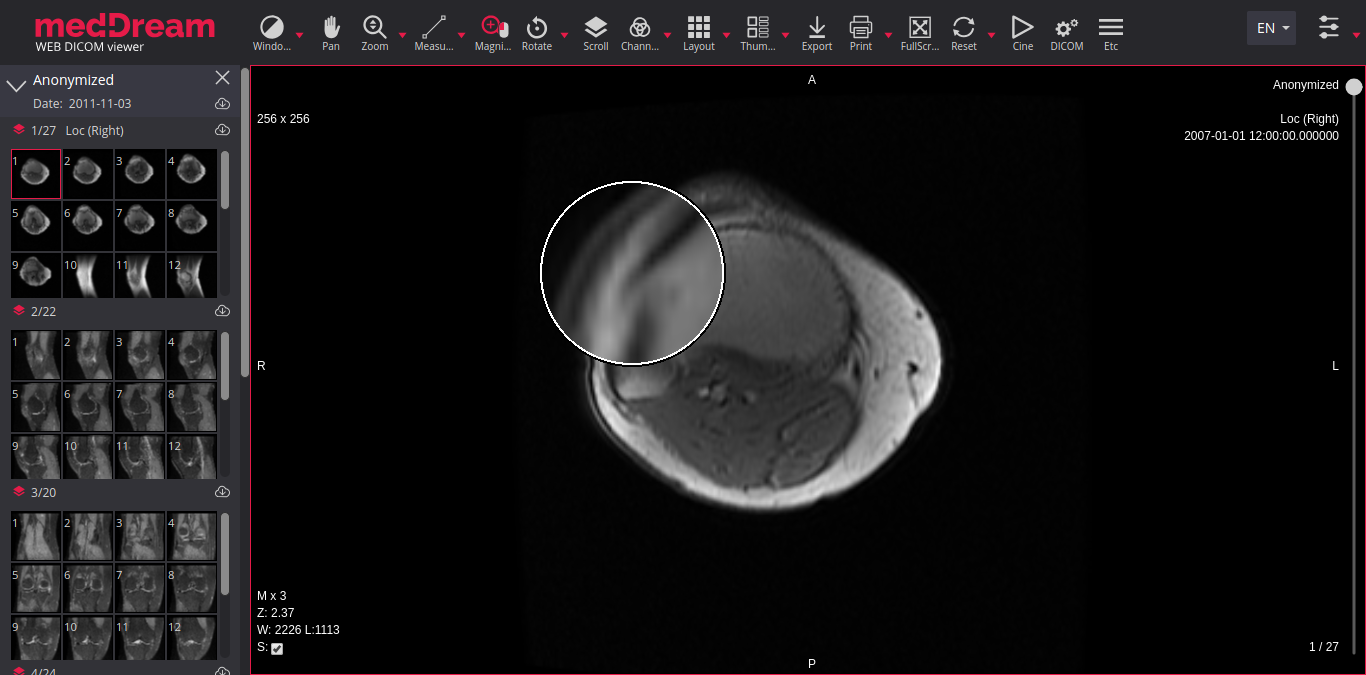
\includegraphics[width=\textwidth]{img/wyswietlanie001.png}
              \caption{Przykład narzędzia Lupa w przeglądarce \href{https://www.softneta.com/products/meddream-dicom-viewer/}{MedDream DICOM Viewer}. Zdjęcie użyte za zgodą \href{https://www.softneta.com/}{Softneta UAB}.}
              \label{fig:wyswietlanie001}
          \end{figure}

    \item Rotacja i odbicia lustrzane
          Możliwość obrócenia obrazu o zadany kąt.
          Oraz możliwość odbicia lustrzanego obrazu w dwóch osiach X i Y.

\end{itemize}

\subsubsection{Analiza parametrów w celu lepszej informacji}

\begin{itemize}
    \item Okienkowanie.
          Termin odnosi się do używania funkcji okna cyfrowego w celu zamiany obrazu danych na obraz monochromatyczny możliwy do wyświetlenia.
          Okienkowanie jest szczegółowo opisane w sekcji \ref{sec:windowing}.

    \item Maski lub nakładki(\fromEng{overlay}).
          Możliwość nałożenia maski, elementu, który będzie przysłaniał fragment obrazu w celu lepszej wizualizacji bądź ukrycie mało wartościowych obiektów, np. tła.
\end{itemize}

\subsubsection{Obsługa wielu plików}

\begin{itemize}

    \item Obsługa DICOMDIR.
          Możliwość wczytania pliku DICOMDIR i wyświetlenie struktury serii badań.

    \item Wczytanie wielu plików i ich połączenie w formie filmu.
          Możliwość wczytania wielu plików z tej samej serii, ułożenia ich według pozycji geometrycznej i wyświetlenia ich jako film.
          Czyli periodyczna podmiana obrazu na obraz następny w serii.

    \item Wyświetlanie wielu obrazów jednocześnie.
          Możliwość wyświetlenia obrazów w postaci kratki, w której każda komórka była by innym obrazem.

          Przykład wyświetlenia wielu obrazów na raz w jednym oknie znajduje się na rysunku \ref{fig:dicomviewer001}

          \begin{figure}[!htbp]
              \centering
              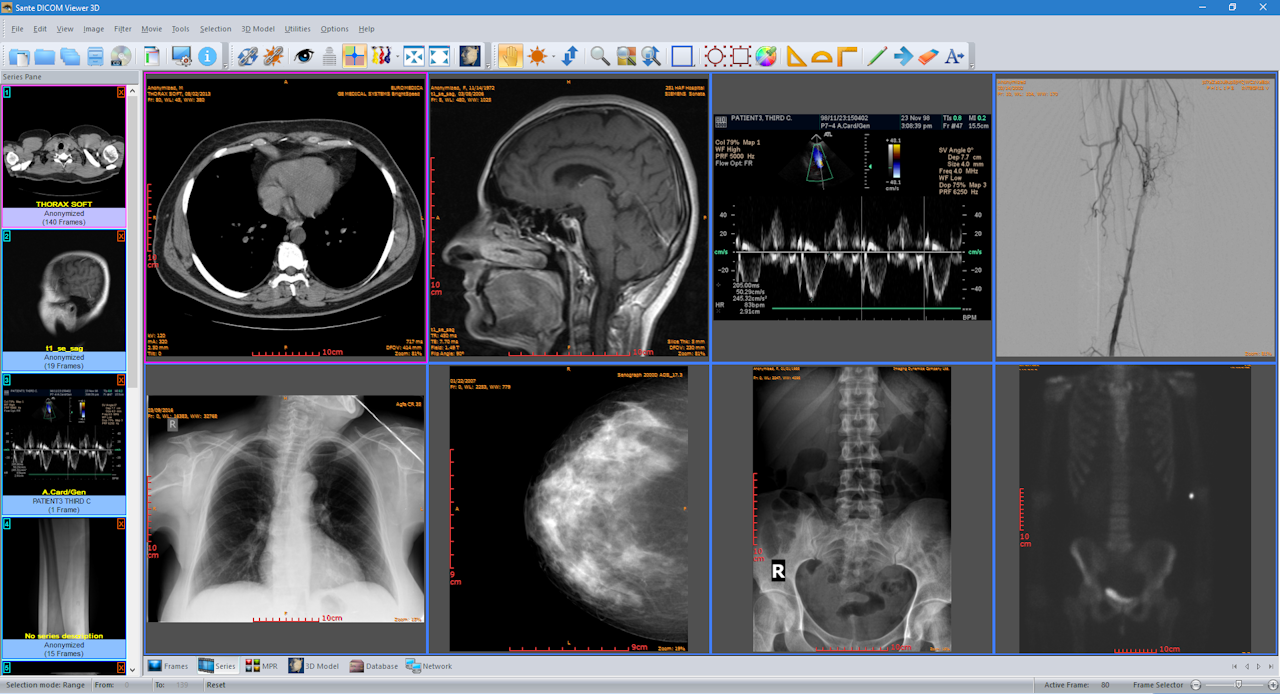
\includegraphics[width=\textwidth]{img/dicom-viewer-001.png}
              \caption{Przykład wyświetlenia wielu obrazów na raz w jednym oknie w przeglądarce \href{https://www.santesoft.com/win/sante-dicom-viewer-3d-pro/sante-dicom-viewer-3d-pro.html}{Sante DICOM Viewer 3D Pro}. Zdjęcie użyte za zgodą \href{https://www.santesoft.com/}{Santesoft}.}
              \label{fig:dicomviewer001}
          \end{figure}
\end{itemize}

\subsubsection{Generowanie obrazów woliumetrcznych}

Jeżeli mamy do dyspozycji wiele obrazów tomograficznych o znanych parametrach to możemy wczytać je, posegregować a następnie wygenerować trój-wymiarowy obiekt a następnie wyświetlić go na ekranie komputera za pomocą trójwymiarowej grafiki komputerowej.

Przykład takiego obrazu znajduje się na rysunku \ref{fig:dicomviewer002}.

\begin{figure}[!htbp]
    \centering
    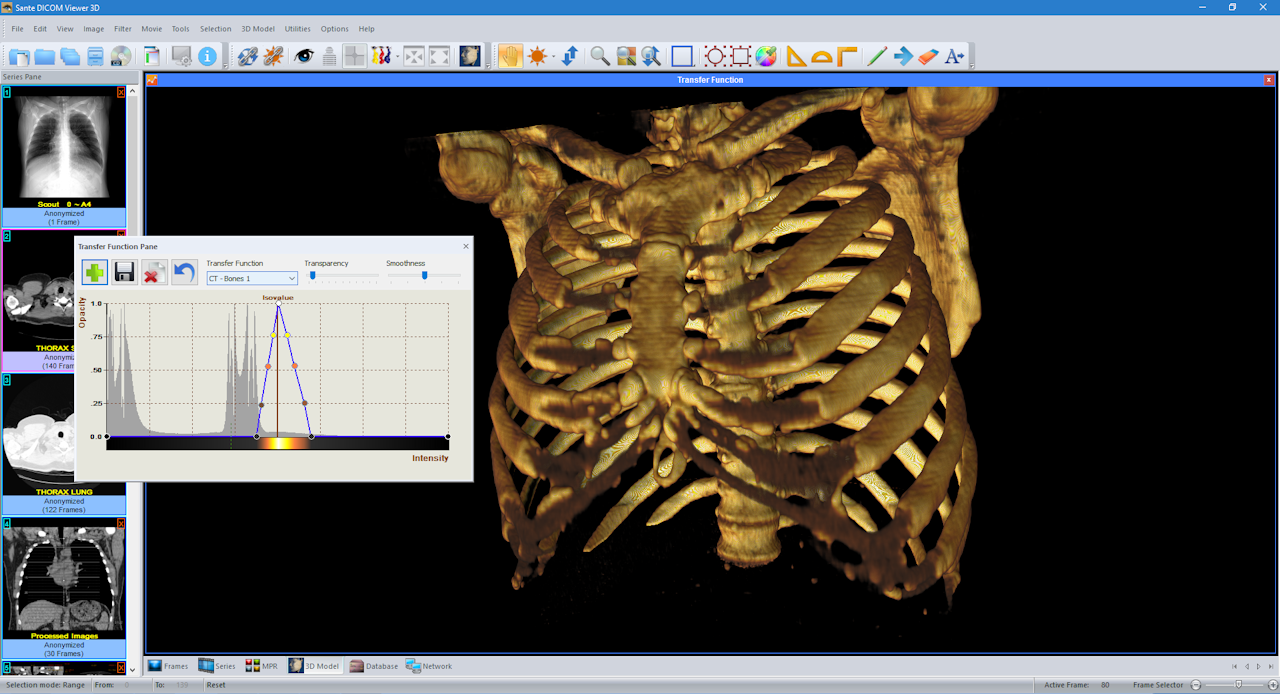
\includegraphics[width=\textwidth]{img/dicom-viewer-002.png}
    \caption{Przykład generowania obrazów 3D z wielu obrazów tomograficznych w przeglądarce \href{https://www.santesoft.com/win/sante-dicom-viewer-3d-pro/sante-dicom-viewer-3d-pro.html}{Sante DICOM Viewer 3D Pro}}
    \label{fig:dicomviewer002}
\end{figure}

\subsubsection{Analiza i przetwarznie danych}

\begin{itemize}
    \item Histogram
          Możliwość wygenerowania histogramu obrazu.

          Histogram to wykres przedstawiający dystrybucje wartości numerycznych obrazu.

    \item Mierzenie obrazu, wykonywanie pomiarów
          Możliwość zmierzenia odległości pomiędzy dwoma punktami przez lekarza lub zmierzenia wielkości/pola zadanego kształtu.

    \item Rekonstrukcja wielopłaszczyznowa.
          Obrazy tomograficzne obrazują przekroje, jeżeli parametry wielkości woksela są dostępne to istnieje możliwość wygenerowania nowego obrazu który byłby obrazem ułożonym w poprzek.

          Przykład generowania rekonstrukcja wielopłaszczyznowej jest pokazany na rysunku \ref{fig:dicomviewer003}

          \begin{figure}[!htbp]
              \centering
              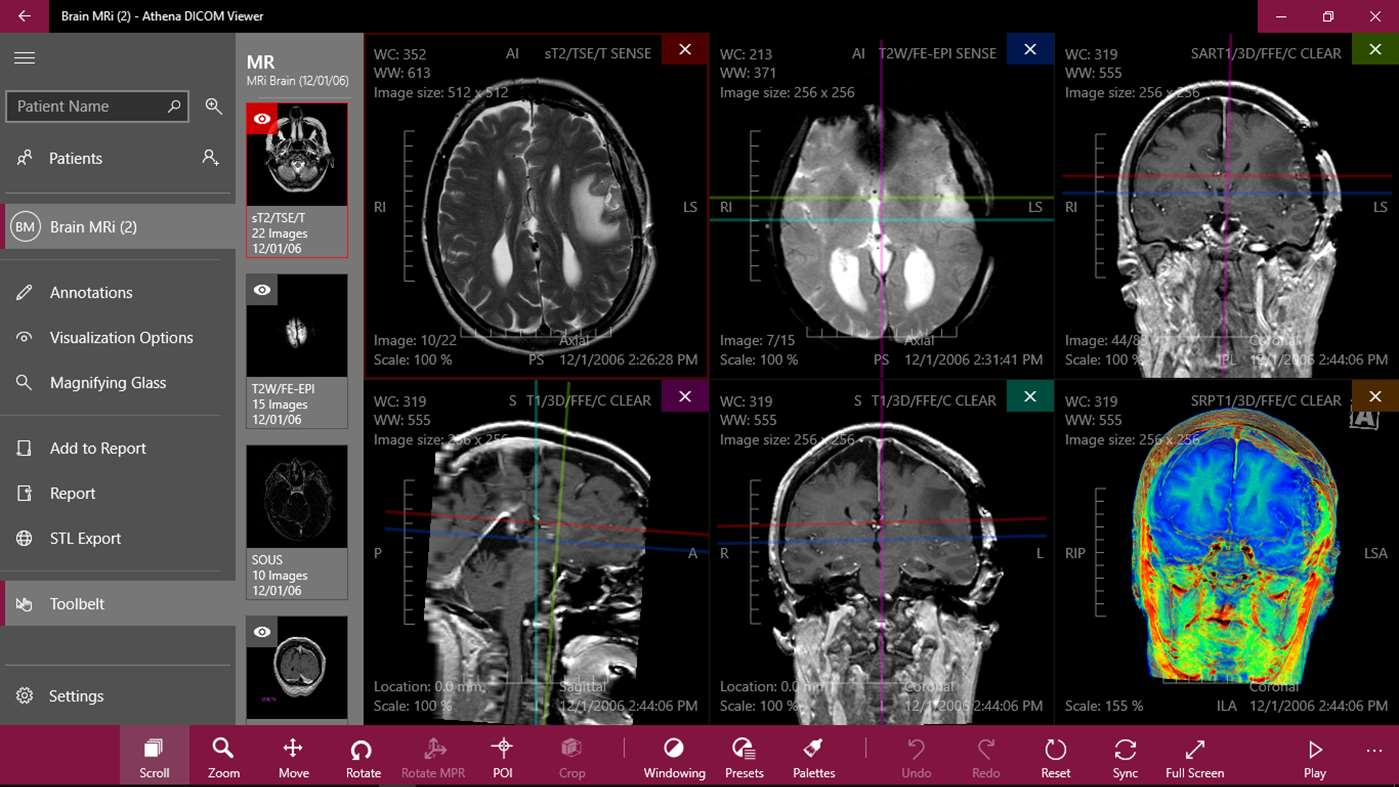
\includegraphics[width=\textwidth]{img/dicom-viewer-003.jpeg}
              \caption{Przykład rekonstrukcji wielopłaszczyznowej w przeglądarce \href{https://athenadicomviewer.com/}{Athena DICOM Viewer}. Zdjęcie użyte za zgodą \href{https://medicalharbour.com/}{Medical Harbour}.}
              \label{fig:dicomviewer003}
          \end{figure}
\end{itemize}

\subsubsection{Edycja danych}

\begin{itemize}
    \item Dodawanie nowych obiektów.
          Możliwość rysowania, dodawania figur geometrycznych lub tekstu przez lekarza i możliwość zapisu tych informacji w pliku DICOM.
          Chodzi tu głównie o szkice i notatki tworzone podczas analizy obrazu przez personel medyczny.

    \item Edycja Parametrów oraz anonimizacja danych.
          Możliwość edycji parametrów w poliku DICOM w różnych celach.
          Najczęściej funkcja jest używana do usuwania danych osobowych pacjenta w celu poźniejszej publikacji obrazu.

\end{itemize}

